\documentclass[12pt]{report}
\usepackage[a4paper, total={7.3in, 9.7in}]{geometry}
\usepackage{amsmath}
\usepackage{upquote}
\usepackage{listings}
\usepackage{xcolor}
\usepackage{titlesec}
\usepackage{amssymb}

\definecolor{backgroundcolor}{rgb}{1, 1, 1}
\definecolor{commentstyle}{rgb}{0.365, 0.422, 0.475}
\definecolor{keywordstyle}{rgb}{0.6, 0.14, 0.576}
\definecolor{numberstyle}{rgb}{0.5, 0.5, 0.5}
\definecolor{stringstyle}{rgb}{0.77, 0.1, 0.08}

\lstdefinestyle{xcodecolor}{
    backgroundcolor=\color{backgroundcolor},   
    commentstyle=\color{commentstyle},
    keywordstyle=\color{keywordstyle},
    numberstyle=\scriptsize\color{numberstyle},
    stringstyle=\color{stringstyle},
    basicstyle=\ttfamily\footnotesize,
    breakatwhitespace=false,         
    breaklines=true,                 
    captionpos=b,                    
    keepspaces=true,                   
    numbersep=5pt,                  
    showspaces=false,                
    showstringspaces=false,
    showtabs=false,                  
    tabsize=2
}

\lstset{style=xcodecolor}

\usepackage[T1]{fontenc}
\usepackage{cascadia-code}
\usepackage{tikz}

% Raised Rule Command:
%  Arg 1 (Optional) - How high to raise the rule
%  Arg 2            - Thickness of the rule
\newcommand{\raisedrule}[2][0em]{\leaders\hbox{\rule[#1]{1pt}{#2}}\hfill}

\newcommand*{\xMin}{0}%
\newcommand*{\xMax}{5}%
\newcommand*{\yMin}{0}%
\newcommand*{\yMax}{5}%

\setlength{\parindent}{0pt}
\titleformat{\section}
  {\normalfont\Large\bfseries}{\thesection}{1em}{}[{\titlerule[0.8pt]}]
\begin{document}

	{\Large
	\textbf{Lighting Trouble}}
	
	\vspace{0.4cm}
	DiPS CodeJam 22\raisedrule[0.25em]{1pt}
	\\
	% document

  \section*{Prompt}
  You're organising a code conference for your school this year, and the volunteers have messed up the lighting. Special lamps are used to light the conference. All the stalls are arranged in a square grid of size $n \times n$, and a lamp covers an entire square. A lamp will light up all stalls in the same row and column. Your volunteers were not organized enough to realize where to place the remaining lamps.\\
  Your job, given the position of the lamps placed so far, is to find out how many stalls have not been lit.

  \subsection*{Input Format}
  \begin{itemize}
    \item The first line of input contains a single integer $n$, denoting the size of the $n \times n$ grid.
    \item The next line contains an integer $m$, denoting the number of lamps used.
    \item The next $m$ lines of input contain 2 integers, giving the row and column of each lamp in the format $(x,y)$.
  \end{itemize}
  \subsection*{Output Format}
  Your output should contain a single integer, denoting the number of stalls (or grid squares) that are not lit.
  \subsection*{Constraints}
  \begin{itemize}
    \item $ 2 \ge n \ge 100 $
    \item $ 1 \ge m \ge 5000 $
  \end{itemize}
  \subsection*{Sample Input/Output}
  \begin{tabular}{ |l|l| } 
    \hline
    \textbf{Input} & \textbf{Output} \\
    {\lstinputlisting{./testCases/input/input00.txt}} & {\lstinputlisting{./testCases/output/output00.txt}} \\ 
    \hline
   \end{tabular}


  \section*{Solution}
  Taking the sample input, let's create a $5\times5$ grid.\\
  
\begin{tikzpicture}
    \foreach \i in {\xMin,...,\xMax} {
      \draw [very thin,gray] (\i,\yMin) -- (\i,\yMax);
    }
    \foreach \i in {\yMin,...,\yMax} {
      \draw [very thin,gray] (\xMin,\i) -- (\xMax,\i);
    }
  \end{tikzpicture}

   Now, let's place the lamps. Taking the sample input, let's place the lamps at $(1, 1)$ and $(3,3)$.\\
  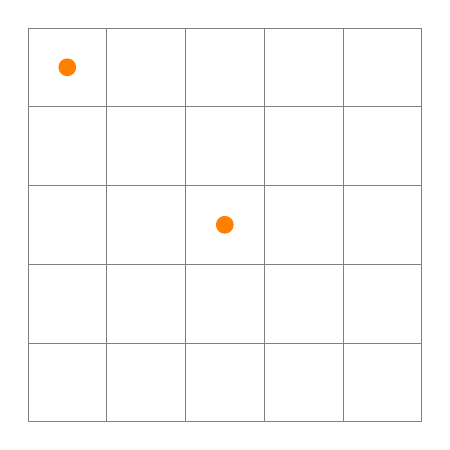
\begin{tikzpicture}
    \foreach \i in {\xMin,...,\xMax} {
      \draw [very thin,gray] (\i,\yMin) -- (\i,\yMax);
    }
    \foreach \i in {\yMin,...,\yMax} {
      \draw [very thin,gray] (\xMin,\i) -- (\xMax,\i);
    }
    
    \filldraw [orange] (0.5,4.5) circle (3pt);
    \filldraw [orange] (2.5,2.5) circle (3pt);
  \end{tikzpicture}

  Now, let's fill up the stalls that are lit by the lamps:\\
  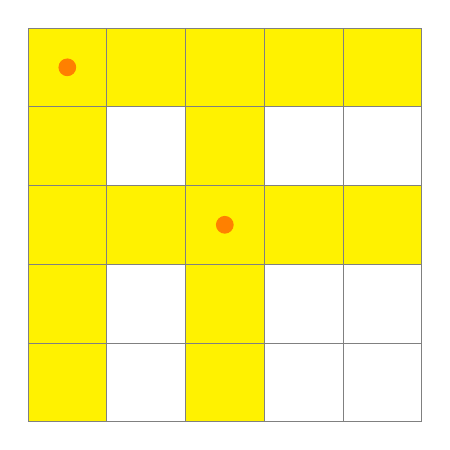
\begin{tikzpicture}
    \fill [yellow] (0,0) rectangle (1,5);
    \fill [yellow] (0,5) rectangle (5,4);
    \fill [yellow] (2,0) rectangle (3,5);
    \fill [yellow] (0,2) rectangle (5,3);

    \foreach \i in {\xMin,...,\xMax} {
      \draw [very thin,gray] (\i,\yMin) -- (\i,\yMax);
    }
    \foreach \i in {\yMin,...,\yMax} {
      \draw [very thin,gray] (\xMin,\i) -- (\xMax,\i);
    }

    \filldraw [orange] (0.5,4.5) circle (3pt);
    \filldraw [orange] (2.5,2.5) circle (3pt);
  \end{tikzpicture}

  We see that there are $9$ stalls (grid squares) that are not lit.

	\section*{Sample Program}
	\lstinputlisting[language=Python]{sampleSolution.py}
	

\end{document}